\chapter{SCIARA-fv3 - Model Formalization}\label{sect:SCIARA_MODEL}

\section{Model Overview}
Sciara-fv3 is the latest release of the Sciara family of
Complex Cellular Automata Models for simulating basaltic
lava flows. As its predecessor, Sciara-fv2, it is
based on a Bingham-like rheology. However, unlike fv2, it explicitly
computes the flow momentum and the time corresponding
to the computational step (CA clock). In formal terms, it is
defined as:
\[
SCIARA-fv3=<R,X,Q,P,\tau,L,\gamma>
\]

where:

\begin{enumerate}
  \item R is the cellular space, the set of square cells that define the
  bi-dimensional finite region where the phenomenon evolves.
  \item X is the pattern of cells belonging to the Moore
neighborhood that influence the cell state change (see fig.
\ref{fig:mooreNeighModel})
  \item \(Q= Q_z \times Q_h  \times Q_T  \times  Q_{\overrightarrow{p}}  \times
  Q_f^9 \times  Q_{\overrightarrow{vf}}^9  \) is the finite set of states,
  considered as Cartesian product of substates. Their meanings are: cell altitude a.s.l.,
cell lava thickness, cell lava temperature, momentum
(both x and y components), lava thickness outflows
(from the central cell toward the adjacent cells) and
flows velocities (both x and y components), respec-
tively;
  \item \(P = w,t_0, P_T,P_d,P_{hc},\delta,\rho,\epsilon,\sigma,c_v\) is the finite set
of parameters (invariant in time and space), whose
meaning is illustrated in Tab. \ref{tab:parameters}; note that \(P_T , P_d\) ,
and \(P_{hc}\) are set of parameters;
\item \(\tau : Q^9 \longmapsto Q\) is the cell deterministic transition
function; it is splitted in \textit{``elementary processes''}  which, are described
in section \ref{sect:ElementaryProcesses};
\item \(L \subseteq R \) specifies the emitted lava thickness from the source
cells (i.e. craters);
\item \(\gamma : Q_h \times \mathbb{N} \longmapsto Q_h\) specifies the emitted
lava thickness from the source cells at each step \(k \in \mathbb{N}\)
  
\end{enumerate}

\begin{figure}
\begin{center}
  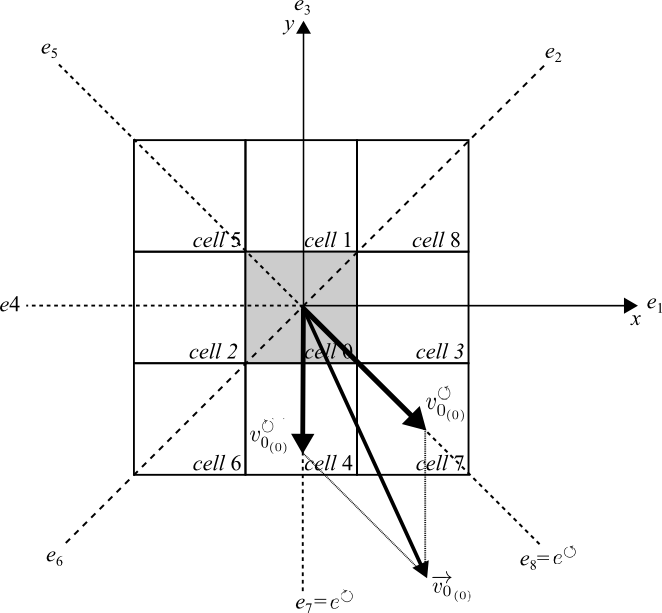
\includegraphics[scale=0.65]{./images/mooreNeighSciaraModel}
  \caption{Example of Moore neighborhood and decomposition of momentum
along the cellular space directions. Cells are indexes from 0 (the central cell,
in grey) to 8. Cells integer coordinates are omitted for a better readability.}
  \label{fig:mooreNeighModel}
\end{center}
\end{figure}


\begin{table}[!t]
% increase table row spacing, adjust to taste
\renewcommand{\arraystretch}{1.3}
% if using array.sty, it might be a good idea to tweak the value of
% \extrarowheight as needed to properly center the text within the cells
\caption{List of parameters of SCIARA-fv3 with values considered for the simulation of the 2006 Etnean lava flow.}
\label{tab:parameters}
\centering
%% Some packages, such as MDW tools, offer better commands for making tables
%% than the plain LaTeX2e tabular which is used here.
\begin{tabular}{l l l l}
\hline
Parameter & Meaning & Unit & Best value\\
\hline
$w$ & Cell side & [m] & 10\\
$t_0$ & Initial CA clock & [s] & 1\\
$t_{\max}$ & Upper value for the CA clock & [s] & 120\\
$P_T$\\
	$\;\;\: T_{sol}$ & Temperature of solidification & [K] & 1143\\
	$\;\;\: T_{vent}$ & Temperature of extrusion & [K] & 1360\\
$P_d$\\
	$\;\;\: dP_{T_{sol}}$ & Dissipation factor at solidification & - & 0.5\\
	$\;\;\: dP_{{T_vent}}$ & Dissipation at extrusion & - & 0.315\\
$P_{hc}$\\
	$\;\;\: hc_{T_{sol}}$ & Critical height at solidification & [m] & 23.066\\
	$\;\;\: hc_{{T_{vent}}}$ & Critical height at extrusion & [m] & 1.014\\
$r$ & Relaxation rate & - & 0.5\\
$\delta$ & Cooling parameter & - & 1.5070\\
$\rho$ & Lava density & [Kg m$^{-3}$] & 2600\\
$\epsilon$ & Lava emissivity & - & 0.9\\
%$\sigma$ & Stephan-Boltzmann constant & [J m$^{-2}$ s$^{-1}$ K$^{-4}$] & $5.68 \cdot 10^{-8}$\\
$c_v$ & Specific heat & [J kg$^{-1}$ K$^{-1}$] & 1150\\
\hline
\end{tabular}
\end{table}

\section{Elementary process}\label{sect:ElementaryProcesses}
\subsection{Elementary process \(\tau_1\): lava flows computation}
The elementary process $\tau_1$ computes lava outflows and their velocities. It is formally defined as:
$$
\tau_1: Q_z^9 \times Q_h^9 \times Q_{\overrightarrow{p}} \to Q_f^9 \times Q_{\overrightarrow{v_f}}^9
$$

Lava flows are computed by a two-step process: the first computes the CA clock,
$t$, i.e. the physical time corresponding to a CA computational step, while the
second the effective lava outflows, $h_{(0,i)}$, their velocities
$v_{f_{(0,i)}}$ and displacements $s_{(0,i)}$ $(i=0,1,...,8)$. The elementary
process $\tau_1$ is thus executed two times, the first one in ``time evaluation
mode'', the second in ``flow computing mode''. Both modes compute the so called
``minimizing outflows'', $\phi_{(0,i)}$, i.e. those which minimize the unbalance
conditions within the neighborhood, besides their final velocities and
displacements. In ``time evaluation mode'', $t$ is preliminary set to a large
value, $t_{\max}$, and the computed displacement, $s_{(0,i)}$, is compared with
the maximum allowed value, $d_{(0,i)}$, which is set to the distance between the
central cell and the neighbor that receives the flow. In case of
over-displacement, the time $t$ must be opportunely reduced in order to avoid
the overflow condition. In case no over-displacement are obtained, $t$ remains
unchanged. Eventually, in ``flow computing mode'', effective lava outflows,
$h_{(0,i)}$, are computed by adopting the CA clock obtained in ``time evaluation
mode'', by guarantying no overflow condition.

\subsubsection{Computation of the minimizing outflows $\phi_{(0,i)}$}\label{sec:min-ouflows}
As in \cite{xxx, xxx}, the initial velocity of the lava inside the cell,
$\overrightarrow{v_{0}}_{_{(0)}}$, is obtained from the momentum components. In
turn, it is decomposed in two components laying over the two directions of the
CA cellular space which are the nearest with respect to
$\overrightarrow{v_{0}}_{_{(0)}}$ itself. These latter directions, which will be
indicated by $e^\circlearrowleft$ and $e^\circlearrowright$, can be found by
moving in counterclockwise and clockwise directions starting from the direction
of $\overrightarrow{v_{0}}_{_{(0)}}$, respectively, as shown in Fig.
\ref{fig:mooreNeighModel}. Thus, if $i$ denotes the $i$-th direction of the cellular
space, $v_{0_{(0)}}^\circlearrowleft$ and $v_{0_{(0)}}^\circlearrowright$ the
modules of the components of $\overrightarrow{v_{0}}_{_{(0)}}$ along the
directions $e^\circlearrowleft$ and $e^\circlearrowright$, respectively, then
the modules of the components of $\overrightarrow{v_{0}}_{_{(0)}}$ along the
directions of the cellular space can be expressed as:
$$ v_{0_{(0,i)}}=
	\begin{cases}
		v_{0_{(0)}}^\circlearrowleft, & \mbox{if }i = e^\circlearrowleft \\
		v_{0_{(0)}}^\circlearrowright, & \mbox{if }i = e	^\circlearrowright \\
		0, & \mbox{otherwise}
	\end{cases}
$$
Moreover, let ${h_k}_{(0,i)} = {v_0}_{(0,i)}^2/2g$ denote the kinetic head associated to the $i$-th component of velocity.

Viscosity effects are modeled in terms of velocity dissipation mechanism, by means of the function $dP$. It depends on temperature and vary according to a power law of the type $\log dP = a+bT$, where $T \in Q_T$ is the lava temperature and $a$ and $b$ are coefficients determined by solving the system (cf. Tab. \ref{tab:parameters}):
$$
\begin{cases}
	\log dP_{T_{sol}} = a+bT_{sol}\\
	\log dP_{T_{vent}} = a+bT_{vent}\\
\end{cases}
$$
Similarly, the relation between critical height and lava temperature can be described by a power law of the kind $\log hc = c+dT$ whose coefficients are obtained by solving the system (cf. Tab. \ref{tab:parameters}):
$$
\begin{cases}
	\log hc_{T_{sol}} = c+dT_{sol}\\
	\log hc_{T_{vent}} = c+dT_{vent}\\
\end{cases}
$$

Before applying the minimization algorithm of the differences for computing the
minimizing outflows, a preliminary control was performed to eliminating cells
that cannot receive lava due to their energy conditions. As in
\cite{Spataro2010}, a topographic correction is considered for flow symmetry
reason. In addition, in Sciara-fv3 the concepts of effective height,
$h_{e_{(0,i)}}$, and apparent height, $h_{a_{(0,i)}}$, was introduced. The first
is the part of $h_{(0)}$ that can really flow out of the cell toward its $i$-th
neighborhood, while the second one is the part which is constrained inside the
cell due to energy conditions. There are three cases (see Fig. \ref{fig:cases}):
\begin{enumerate}
\item if $z_{(0)} + h_{k_{(0,i)}} + h_{(0)} \leq z_{(i)} + h_{(i)}$, then \\
$\begin{cases}
	h_{e_{(0,i)}} = 0\\
	h_{a_{(0,i)}} = h_{(0)}\\
\end{cases}$
\item if $z_{(0)} + h_{k_{(0,i)}} < z_{(i)} + h_{(i)} < z_{(0)} + hk_{(0,i)} + h_{(0)}$, then \\
$\begin{cases}
	h_{e_{(0,i)}} = (z_{(0)} + h_{k_{(0,i)}} + h_{(0)}) - (z_{(i)} + h_{(i)})\\
	h_{a_{(0,i)}} = h_{(0)} - h_{e_{(0,i)}}\\
\end{cases}$
\item if $z_{(i)} + h_{(i)} \leq z_{(0)} + h_{k_{(0,i)}}$, then \\
$\begin{cases}
	h_{e_{(0,i)}} = h_{(0)}\\
	h_{a_{(0,i)}} = 0\\
\end{cases}$
\end{enumerate}
Thus, if denoting with $\theta_{(0,i)} = \arctan ((z_{(0)} + h_{a_{(0,i)}} + h_{e_{(0,i)}}/2) - (z_{(i)} + h_{(i)}))$ the slope angle between the central cell and its $i$-th neighbor (see Fig. \ref{fig:cases}), according to the concept of critical height, the cells for which
$$
h_{e_{(0,i)}} \leq hc \cos \theta_i
$$
are eliminated and cannot receive flow.

The minimization algorithm of the differences is therefore applied to the following quantities, in order to compute the minimizing outflows:

\begin{tabular}{l}
$u_{(0)} = z_{(0)}$\\
$m = h_{(0)}$\\
$u_{(i)} = z_{(i)} + h_{(i)}$
\end{tabular}

The application of the algorithm determines the computation of the minimizing flows, $\phi_{(0,i)}$, from the central cell to the $i$-th neighbor, where $\phi_{(0,0)}$ represents the residual flow which does not leave the cell. Eventually, final velocities and displacements are computed. As a first step, final velocities are computed for each outflow $\phi_{(0,i)}$ $(i=1,2, \ldots, 8)$, by taking into account dissipation:
$$
v_{f_{(0,i)}} = (v_{0_{(0,i)}} + a t)(1-dP)
$$
Here, $a = g \sin \theta$ is the acceleration of gravity, and does not take into account dissipation, which is modeled by the function $dP$. Instead, the final velocity of $\phi_{(0,0)}$ is computed as:
$$
v_{f_{(0,0)}} = v_{0_{(0)}}(1-dP)
$$
In order to compute the displacement, a mean acceleration is computed, which also takes into account dissipation effects: $\overline{a} = (v_{f_{(0,i)}} - v_{0_{(0,i)}})/t$. Therefore, the displacements $s_{(0,i)}$ $(i = 1,2, \ldots, 9)$ are computed as:
$$
s_{(0,i)} = v_{0_{(0,i)}} t + \frac{1}{2} \overline{a} t^2
$$
while, a null displacement is assigned to $\phi_{(0,0)}$:
$$
s_{(0,0)} = 0
$$
since, even if in the real case a movement can occur, inside the discrete context of the cellular space, it is always located at the center of the cell. This is a model simplification which is much more correct as the smaller the size of the cell is.

\begin{figure}[!t]
\centering
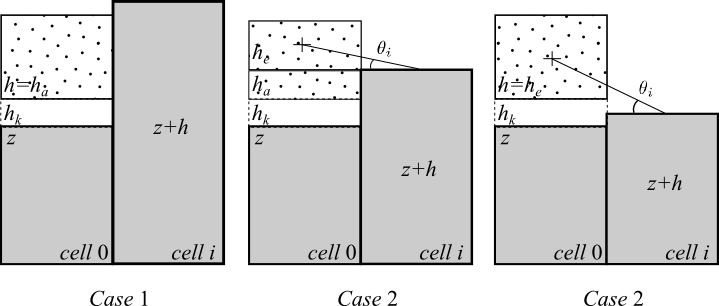
\includegraphics[scale=0.8]{./images/fig2PDP}
\caption{Cases in which the generic neighbor (\textit{cell} $i$) is
eliminated or not eliminated by the minimization algorithm of the difference. If the neighbor is eliminated (\textit{Case} 1), the overall amount of debris inside the central cell is considered as apparent ($h=h_a$), and can not generate an outflow. If the neighbor is not eliminated (\textit{Case} 2 and 3), a part (\textit{Case} 2) or the entire amount of debris (\textit{Case} 3) on the central cell is considered effective ($h \geq h_e$) and can generate outflows. Note that the slope angle $\theta$, considered in the critical height computation, is also shown.}
\label{fig:cases}
\end{figure}

\subsubsection{Time evaluation}\label{sect:modeltimeEvaluation}
Once the minimizing outflows are computed, the CA clock can be determined. As stated above, when $\tau_1$ is executed in ``time evaluation mode'', $t$ is preliminary set to a large value, $t_{\max}$. As a consequence, the computed displacements, $s_{(0,i)}$, can overcome the maximum allowed distance, $w$, i.e. the distance between the central cell and the neighbor that receive the flow. In case of over-displacement, i.e. $s_{(0,i)} > w$, the time $t$ must be opportunely reduced in order to avoid the overflow. The new value of $t$ is determined as follows:

%As a consequence, the computed displacements, $s_{(0,i)}$, can overcome the maximum allowed distance, $d_{(0,i)}$, which is set equal to the distance between the central cell and the neighbor that receive the flow:
%$$
%d_{(0,i)}=
%	\begin{cases}
%		w, & \mbox{if }i \in \{1,2,3,4\} \\
%		w \sqrt{2}, & \mbox{otherwise }\\
%	\end{cases}
%$$
%In case of over-displacement, i.e. $s_{(0,i)} > d_{(0,i)}$, the time $t$ must be opportunely reduced in order to avoid the overflow. The new value of $t$ is determined as follows:

\begin{itemize}
%\item for each minimizing flow, $\phi_{(0,i)}$, a new time, $t_{(0,i)}$, is computed by imposing $s_{(0,i)} = d_{(0,i)}$ and by solving the equation with respect to $t$:
%$$
%t_{(0,i)} = t = \frac{ - v_{0_{(0,i)}} + \sqrt{v_{0_{(0,i)}}^2 + 2 \overline{a} d_{(0,i)}} }{\overline{a}}
%$$
%so that overflow is avoided between the central cell and its $i$-th neighbor;

\item for each minimizing flow, $\phi_{(0,i)}$, a new time, $t_{(0,i)}$, is computed by imposing $s_{(0,i)} = w$ and by solving the equation with respect to $t$:
$$
t_{(0,i)} = t = \frac{ - v_{0_{(0,i)}} + \sqrt{v_{0_{(0,i)}}^2 + 2 \overline{a} w} }{\overline{a}}
$$
so that overflow is avoided between the central cell and its $i$-th neighbor;


\item a new time, $t_j$, is computed in order to avoid overflow conditions along all the neighborhood as:
$$
t_c = \min_{i=1,2, \ldots ,8} t_{(0,i)}
$$
so that overflow is avoided in all the neighborhood;

\item a new minimal time, $t_{opt}$, is computed as:
$$
t_{opt} = \min_{c \in R} t_{c}
$$
in order to avoid overflow conditions over all the cellular space $R$;

\item $t_{opt}$ is multiplied by a relaxation rate factor, $0 < r \leq 1$, for smoothing the phenomenon, and the new CA clock, $\overline{t}$, is obtained:
$$
\overline{t} = t_{opt} r
$$
\end{itemize}

\subsubsection{Outflows computation}
In ``flow computing mode'', minimizing outflows, $\phi_{(0,i)}$, are re-computed by considering the new CA clock $\overline{t}$. Subsequently, lava outflows, $h_{(0,i)}$, are computed proportionally to the displacement, by simply multiplying the minimizing outflow by the ratio between the actual displacement and the maximum allowed:
$$
%h_{(0,i)} = \phi_{(0,i)} \frac{ s_{(0,i)} }{ d_{(0,i)} }
h_{(0,i)} = \phi_{(0,i)} \frac{ s_{(0,i)} }{ w }
$$
Final velocity and displacement are computed as in Section \ref{sec:min-ouflows}.



\subsection{Elementary process $\tau_2$: updating of mass and
momentum}\label{sect:sciaraModelTau2} The elementary process updates lava
thickness and momentum.
It is formally defined as:
$$
\tau_2: Q_f^9 \times Q_{\overrightarrow{v_f}}^9 \to Q_h \times Q_{\overrightarrow{p}}
$$
Once the outflows $h_{(0,i)}$ are known for each cell $c \in R$, the new lava thickness inside the cell can be obtained by considering the mass balance between inflows and outflows:
$$
h_{(0)} = \sum_{i=0}^9 (h_{(i,0)} - h_{(0,i)})
$$

Moreover, also the new value for the momentum can be updated by accumulating the contributions given by the inflows:
$$
\overrightarrow{p}_{(0)} = \sum_{i=0}^9 h_{(i,0)} \overrightarrow{v_f}_{_{(i,0)}}
$$
%while its components along the $x$ and $y$ directions can be simply obtained as:
%$$
%p_{x_{(0)}} = \sum_{i=0}^9 h_{(i,0)} v_{(i,0)} \cos \alpha_{(i,0)}
%$$
%$$
%p_{y_{(0)}} = \sum_{i=0}^9 h_{(i,0)} v_{(i,0)} \sin \alpha_{(i,0)}
%$$	
%being $\alpha_{(i,0)}$ the angle which defines the direction of the velocity of the $i$-th inflow, $h_{(i,0)}$.

\subsection{Elementary process $\tau_3$: temperature variation and lava
solidification}\label{sect:temperatureDrop}

$$
\tau_3: Q_f^9 \times Q_T^9 \to Q_T \times Q_h
$$

As in the elementary process $\tau_1$, a two step process determines the new
cell lava temperature. In the first one, the temperature is obtained as weighted
average of residual lava inside the cell and lava inflows from neighboring ones:
$$
\overline{T} = \frac{ \sum_{i=0}^8 h_{(i,0)} T_i } { \sum_{i=0}^8 h_{(i,0)} }
$$ A further step updates the calculated temperature by considering thermal
energy loss due to lava surface radiation \cite{Park1984}:
$$ T = \frac{\overline{T}}  { \sqrt[3]{1 + \frac{3\overline{T}^3 \epsilon \sigma
\overline{t} \delta}{\rho c_v w^2 h}} } $$ where $\epsilon$, $\sigma$,
$\overline{t}$, $\delta$, $\rho$, $c_v$, $w$ and $h$ are the lava emissivity,
the Stephan-Boltzmann constant, the CA clock, the cooling parameter, the lava
density, the specific heat, the cell side and the debris thickness, respectively
(see Tab. \ref{tab:parameters}). When the lava temperature drops below the
threshold $T_{sol}$, lava solidifies. Consequently, the cell altitude increases
by an amount equal to lava thickness and new lava thickness is set to zero.

Lava flows are computed by a two-step process: the first computes the CA clock, $t$, i.e. the physical time corresponding to a CA computational step, while the second the effective lava outflows, $h_{(0,i)}$, their velocities $v_{f_{(0,i)}}$ and displacements $s_{(0,i)}$ $(i=0,1,...,8)$. The elementary process $\tau_1$ is thus executed two times, the first one in ``time evaluation mode'', the second in ``flow computing mode''. Both modes compute the so called ``minimizing outflows'', $\phi_{(0,i)}$, i.e. those which minimize the unbalance conditions within the neighborhood, besides their final velocities and displacements. In ``time evaluation mode'', $t$ is preliminary set to a large value, $t_{\max}$, and the computed displacement, $s_{(0,i)}$, is compared with the maximum allowed value, $d_{(0,i)}$, which is set to the distance between the central cell and the neighbor that receives the flow. In case of over-displacement, the time $t$ must be opportunely reduced in order to avoid the overflow condition. In case no over-displacement are obtained, $t$ remains unchanged. Eventually, in ``flow computing mode'', effective lava outflows, $h_{(0,i)}$, are computed by adopting the CA clock obtained in ``time evaluation mode'', by guarantying no overflow condition.

